\documentclass[11pt, a4paper]{article}

\usepackage{enumitem}
\usepackage{mathtools}
\usepackage{hyperref}
\usepackage{tikz}
\usepackage{fancyvrb}
%\usepackage[top=1in, bottom=0.4in]{geometry}

\pagenumbering{gobble}

\begin{document}

  \title{Addressing cold start in music recommendation}
  \author{Ioannis Gakos, Wiktor Grajkowski - Group 37}
  \date{16th April 2016}
  \maketitle

  \section{Introduction}
    The shift of the music industry towards the Web has made music
    recommendation a relevant problem which solution could radically improve
    users' experience. However, in the absence of usage data, existing methods,
    such as collaborative filtering, fall short in taking effective decisions
    for new and unpopular content.
    \\ \\
    \noindent
    This project aims to build a music recommendation system using
    Convolutional Neural Network (CNN). CNNs have been widely used in
    applications such as image recognition and recommendation systems. Our
    design is based on recent work of Aaron van den Oord et al. on music
    recommendation \cite{deep-content-based-music-recommendation} using deep
    CNNs and on Dieleman's post \cite{spotify-dieleman} on the implementation
    and architecture details of such CNN built during his internship at
    Spotify.
    \\ \\
    \noindent
    We built a system that addresses the cold start problem for both new users
    and music content. The users give a single preferred track as input, based
    on which a shuffled playlist with similar music is generated. Newly
    imported music content, without previous usage related feedback, can be
    classified based solely on its frequency spectrum. It is achieved by
    propagating the spectrum through a CNN trained to predict latent
    representations obtained from a separate, tag based model. The tags and
    audio samples were obtained from the MagnaTagATune open dataset consisting
    of 26,000 user annotated audio clips.

  \section{Related Work}
    Traditional content recommendation systems rely on user usage data to make
    decisions. Behavior patterns between users, are used by collaborative
    filtering methods to make recommendations about various types of content.
    However, collaborative filtering suffers from the cold start, i.e. ability
    to recommend under the lack of usage data such as user's music taste or
    songs frequently listened together.
    \noindent
    Latent vectors can be used as compact representation of the user's
    preferences correlated with other characteristics of the items. Predicting
    these vectors for new music content based only on metadata such as the artist's
    name or album is often impossible. Using audio content to predict latent factor
    vectors can bridge the semantic gap between the characteristics of an audio
    track and the user's preferences. A\"{a}ron van den Oord et al.
    \cite{deep-content-based-music-recommendation} converted existing usage
    data, present in the Million Song Dataset (MSD), to the latent vector space
    using Weighted Matrix Factorization and trained a CNN using these vectors
    to minimize the Mean Squared Error of the predicted latent vectors of audio
    samples. Visualization of their qualitative evaluation is depicted in
    Figure 1. In order to train their CNN, they used the Million Song Dataset,
    a much larger collection than the MagnaTagATune dataset that we used.

    \begin{figure}
      \centering
      \rotatebox{0}{\scalebox{1}{
        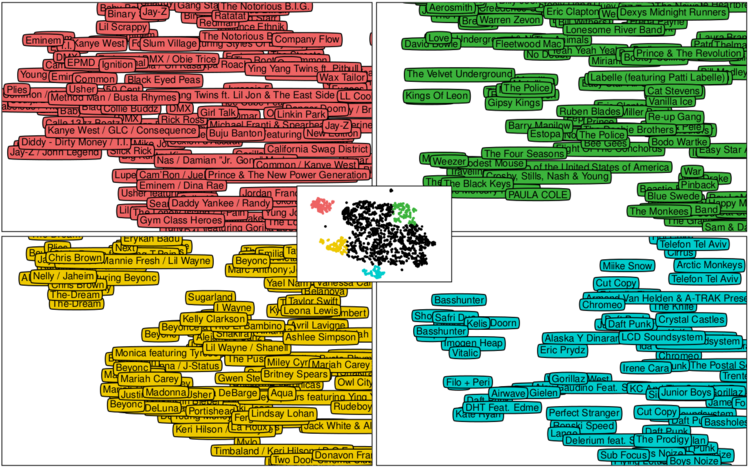
\includegraphics[
          width=12cm,height=12cm,keepaspectratio]{latent-space-visualization.png}}}
      \caption{Visualization of the artist classification using latent factors
        predicted from audio \cite{deep-content-based-music-recommendation}}
    \end{figure}

  \section{Dataset}
    In order to train the CNN and tag based model, we used the MagnaTagATune
    dataset, which was made available by the Magnatune label for the research
    community. The data was collected using the TagATune game where users
    annotated audio tracks with audio relevant tags.
    \\ \\
    \noindent
    The dataset consists of approximately 26,000 29 seconds long music samples
    encoded in 16 kHz, 32kbps, mono mp3, generously contributed by John
    Buckman, the founder of every MIR researcher's favorite label - Magnatune.
    Each of them is annotated with a combination of 188 tags such as
    "orchestral", "classical", "punk", "slow", "blues", "rock" etc. It also
    contains music similarity annotations in the form of triples where given a
    triple of songs (A, B, C), metrics of how many players have flagged the
    song A, B or C as most different from the others.
    \\ \\
    \noindent
    While preprocessing the dataset to build the latent vector space
    representation of the tags and extract the mel spectrograms of the samples
    we found that approximately 5000 samples had zero tag annotations and 3 of
    the mp3 clips were 0 bytes long, which as explained in the implementation
    details section we had to exclude from the final training dataset
    \cite{magnatagatune}.

  \section{Design architecture}
    Due to our prior lack of experience in the field we decided to follow
    and later vary an existing and tested to be working CNN architecture, in
    particular that described by Sander Dieleman in his blog post
    \cite{spotify-dieleman}
    \\ \\
    \noindent    
    In order to be able to suggest songs similar to that provided by the user
    we rely solely on the audio content of the supplied track. The exact format
    used as an input to the networ is a mel spectrogram of a 29 s long sample
    of the track. Spectrogram captures how the frequency spectrum of the clip
    changes in time by performing fourier transform on short (order of ms),
    overlapping windows. The frequency is log scaled (using mel scale) to reduce
    the dimensionality which speeds up the network training phase. We have
    experimented with different settings for the spectorgram parameters. Figure
    2 shows two spectrograms of the same song one with windows size of 512
    samples and one with 3072 samples. It can be seen that the smaller window
    results in better time resolution and more blured frequency, where the
    larger window has better frequency resolution, which can be seen especially
    for low frequencies, but is more blured in time domain. The size of the
    window also determines the number of frames needed to represent the audio
    clip and we have chosen window of size 3116 as it produced the same number
    of frames as in Dieleman architecture.
    \\ \\
    \noindent
    We fed the spectrograms into a neural network consisting of 3 convolutional
    layers that learn to extract time dependent features interleaved with
    max pooling layers that reduce the time dimension for faster learning and
    add invariance so that small changes in the exact position of the feature
    do not matter. After the convolutional layers, two fully connected, global
    pooling (dense) layers are included to gather statistics about the learned
    filters across the full time dimension as overall in order to classify a
    song the exact position of the features should not matter as much as the
    fact that they are present. Finally, the output layer returns the latent
    vector representation of the song.
    \\ \\
    \noindent
    The network is trained to minimise the mean squared error between the
    prediction (output of the network) and ground truth data obtained from
    a separate, tag based model. To build the latent representation from the
    tags we use doc2vec which is an extension to word2vec algorithm that treats
    the set of user annotations for a particular clip as ``bag of words'' and 
    projects them into one multidimensional space. We chose this model as it
    provides needed functionality and hides all the details so we can focus
    on the neural network implementation.
    \\ \\
    \noindent
    The CNN layers are depicted in Figure 3. The first layer shows the
    spectrogram with the red rectangles depicting the convolutions. The red
    triangles represent the downsampling by max pooling. We used pool size
    of 4x1 between the first and second layer for greater dimension reduction
    and size of 2x1 between the rest of layers. Max pool of size 4x1 means that
    we look at a particular frequency bin in 4 consequtive time frames and keep
    only the maximum value from the set of values in the pool. We did not
    include the L2 normalization global pooling as we could not manage to
    implement it.
    \\ \\
    \noindent
    In order to make recommendations we calculate the euclidean distance of the
    predicted latent representation of the input song to all of the clips
    present in our dataset and choose the top ten results that we present to
    the user along with their corresponding tags.

    \begin{figure}
      \centering
      \rotatebox{0}{\scalebox{1}{
        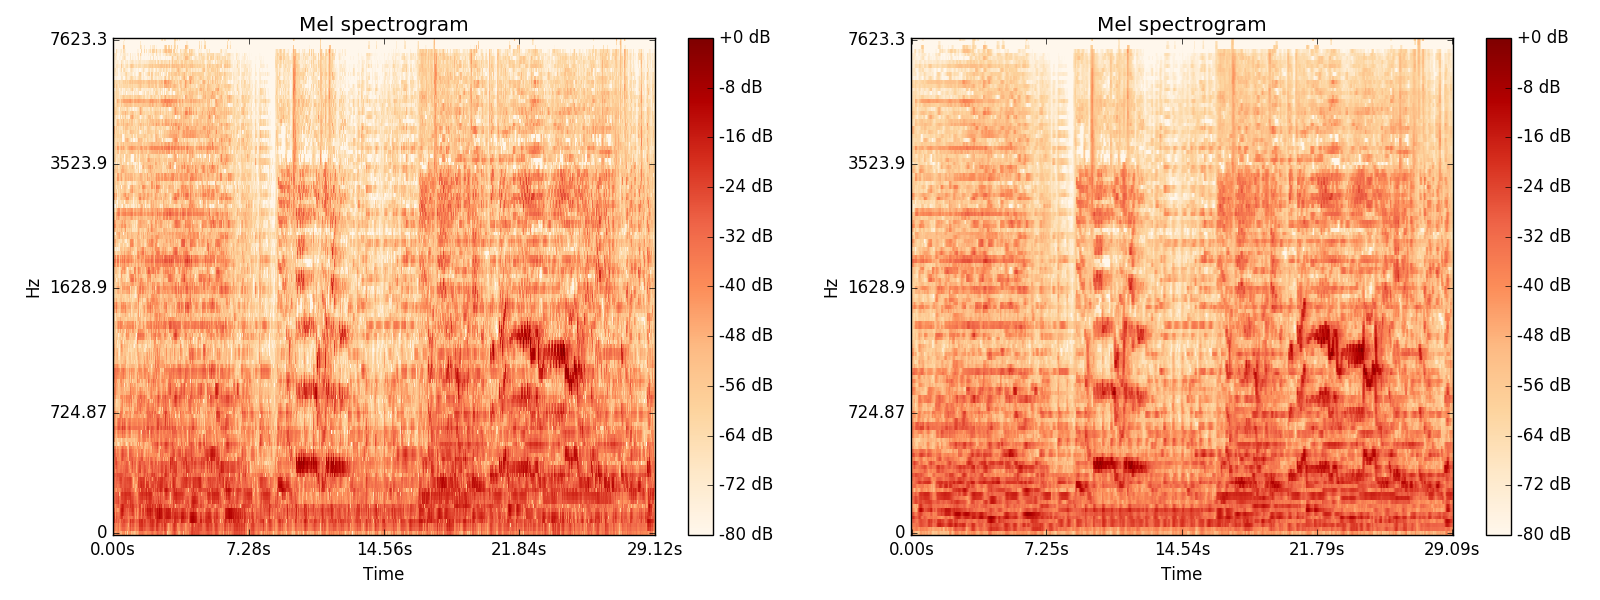
\includegraphics[
          width=12cm,height=12cm,keepaspectratio]{spectrograms.png}}}
      \caption{Comparison of spectrograms with window size of 512 samples
          (left) and 3072 samples (right)}
    \end{figure}

    \begin{figure}
      \centering
      \rotatebox{0}{\scalebox{1}{
        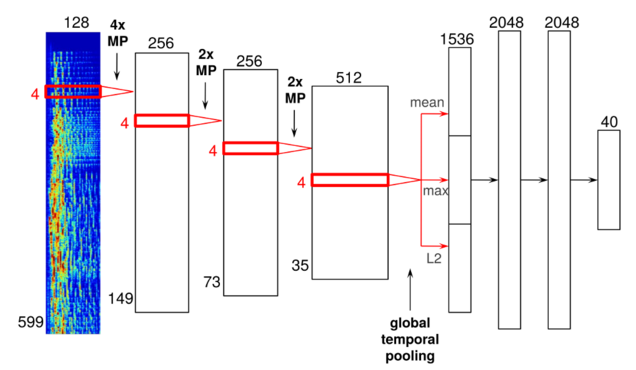
\includegraphics[
          width=12cm,height=12cm,keepaspectratio]{cnn-architecture.png}}}
      \caption{Neural network architecture we implemented that closely follows
        one of the architectures Dieleman experimented with.
        (\url{ http://benanne.github.io/images/spotify\_convnet.png})}
    \end{figure}

  \section{Implementation Details}
    In order to facilitate building and training the Convolutional Neural
    Network we used the Lasagne, the most mature and active lightweight library
    currently available in the community \cite{lasagne}. The library provides
    already implemented layers such as 2D Convolutional and Fully connected
    ones (DenseLayer) that we used in our implementation.
    \\ \\
    \noindent
    Before training the network, we applied a lot of preprocessing on the
    dataset we used resulting in a dataset of 21642 training, validation and 
    testing samples. The preprocessing included exclusion of samples from the
    dataset that had no tags attached in order to avoid pushing the training
    towards overfitting on tracks with no feature information available.
    \\ \\
    \noindent
    To move from tags to the latent vector space and this way build the ground
    truth model, we used the Doc2Vec model that the network used to minimize
    its predictions' error \cite{doc2vec}. In order to prepare samples for
    training we used the librosa library \cite{librosa} to extract the mel
    spectrograms of all of the samples included in the dataset, a rather time
    consuming process.
    \\ \\
    \noindent
    Our implementation provides a full working flow, meaning that it supports
    all the steps from preprocessing the dataset up to the point of getting
    a list of the 10 most similar tracks given a target from the dataset. It
    also supports multiple execution environments based on the computational
    power available. We did that because we needed to be able to quickly switch
    from our local development environments to the production one that we used
    for training, an EC2 GPU instance running on AWS cloud.
    \\ \\
    \noindent
    All the code and documentation for the project is hosted on github:\\
    https://github.com/iogakos/shufl
      
  \section{Tests and Results}
    While evaluating our model we tried several test samples and realized that
    our model learns some filters but is biased towards the majority of the tones
    in the dataset which includes mostly classical and instrumental music. We
    believe that the MagnaTagATune dataset does not contain too many samples to
    build a really smart network, though it contained enough to build a prototype 
    / proof of concept which was mainly the purpose of this project.
    \\ \\
    \noindent
    Following we query a track that contains mostly instrumental music and more
    specifically the violin instrument. On top you can see the difference between
    the ground truth (real) and the predicted vector from our model, translated
    into the most similar clip ids with their corresponding tags. Though there are
    few false positive results in the predicted results, the list includes a bias
    towards specific harmonics of violin and its similar instrument cello.
    \begin{Verbatim}[xleftmargin=.5in]
    $ python shufl.py -m user -t CLIP_2
    Loading local configuration
    Loading data...
    Building model and compiling functions...
    Entered user mode
    Calculating closest vectors for CLIP_2
    predict   real      diff
    1.028302  1.157982 -0.129680
    1.024865  1.179301 -0.154436
    1.043520  0.993746  0.049774
    1.111636  1.137265 -0.025629
    1.003731  1.011692 -0.007962
    0.978039  0.959152  0.018886
    1.160172  0.915732  0.244440
    1.090362  1.164641 -0.074278
    1.081008  0.963084  0.117924
    1.057104  1.043706  0.013398
    1.125383  1.129928 -0.004545
    0.964547  1.072555 -0.108007
    1.058979  1.085058 -0.026079
    0.961544  1.260793 -0.299249
    0.956261  1.242349 -0.286088
    1.011432  1.115816 -0.104384
    1.043542  1.023080  0.020463
    1.046357  0.873973  0.172384
    0.982478  0.969929  0.012549
    0.986319  1.045492 -0.059173
    1.091416  0.902382  0.189034
    0.955335  0.897604  0.057731
    1.080080  0.856658  0.223423
    1.114109  1.112599  0.001510
    1.015443  1.227245 -0.211801
    1.089310  0.857949  0.231361
    1.061282  1.006443  0.054839
    1.042227  1.082391 -0.040164
    0.937966  1.278669 -0.340702
    1.035637  1.115713 -0.080076
    1.058759  1.073235 -0.014475
    1.079493  1.118363 -0.038870
    0.972410  0.982463 -0.010053
    0.932406  0.888498  0.043908
    1.018215  1.063535 -0.045320
    1.103993  1.047916  0.056076
    1.082609  0.738551  0.344058
    1.061711  0.954425  0.107286
    1.061112  1.147689 -0.086577
    1.117326  1.278288 -0.160962
    query: CLIP_2'classical','strings','opera','violin'
    CLIP_52084 'violin','cello'
    CLIP_15381 'violin','cello'
    CLIP_26669 'rock','metal'
    CLIP_25231 'dance','techno','beat'
    CLIP_53212 'classical','strings','violin','cello'
    CLIP_10202 'violin','cello'
    CLIP_29177 'violin','cello'
    CLIP_28628 'dance','techno','beat'
    CLIP_51984 'classical','strings','violin','cello'
    CLIP_51680 'classical','strings','violin','cello'
    \end{Verbatim}

    \noindent
    We present the same effect from another clip that contains both violin and
    cello and for clarity we suppressed the vector distances. The model seems to
    be able to understand the violin's harmonics but is not that fluent with
    finding combinations of the instrument with cello.
    \\ \\

    \begin{Verbatim}[xleftmargin=.5in]
    query: CLIP_94 'novoice','classical','strings',
        'violin','cello','soft'

    CLIP_18510 'classical','strings','violin'
    CLIP_17131 'classical','strings','violin'
    CLIP_42243 'classical','strings','violin'
    CLIP_29858 'classical','strings','violin'
    CLIP_10204 'classical','strings','violin','cello'
    CLIP_33383 'classical','strings','violin','cello'
    CLIP_24353 'classical','strings','violin'
    CLIP_2544 'classical','strings','violin'
    CLIP_27686 'classical','strings','violin'
    CLIP_51984 'classical','strings','violin','cello'
    \end{Verbatim}

    \noindent
    On the other hand, we find the network struggles in understanding frequency
    spectrums of loud and fast music such as heavy metal. We believe this is
    because of the nature of the dataset of mostly containing instrumental and
    classical music. For example, 4395 out of ~26000 tracks contain the tag
    'classical' whereas only 522 of them contain the tag 'metal' (276 contain the
    tag 'heavy'). This effect is present in the following query, where the list
    contains very few 'rock' and 'metal' tracks, while being biased against
    instrumental music on the bottom half the list.

    \begin{Verbatim}[xleftmargin=.5in]
    query: CLIP_188'heavy','guitar','loud','heavy_metal',
        'man','rock','metal'
    CLIP_26669 'rock','metal'
    CLIP_37278 'dance','techno','beat'
    CLIP_41027 'drums','electronic','fast','techno','beat'
    CLIP_26694 'rock','metal'
    CLIP_51984 'classical','strings','violin','cello'
    CLIP_53212 'classical','strings','violin','cello'
    CLIP_48219 'electronic','fast','techno','beat'
    CLIP_51680 'classical','strings','violin','cello'
    CLIP_54825 'classical','strings','violin','cello'
    CLIP_6862 'classical','violins','strings'
    \end{Verbatim}

  \section{Time Constraints}
    Due to very busy end of term and other University comittments we had very
    limited time to work on the project. The entire implementation including
    the steep learning curve took us one week. Had we had more time we would
    like to look further into why our CNN model is not learning to generalize.
    One of the reasons could be a tiny architecture detail such as the choice
    of nonlinearity for the activation function, dropout probablility or
    learnig rate. Aternatively we suspect the very narrow range of values in
    the latent representation obtained from doc2vec model could make it hard
    for the network to learn the exact values. If that was the case
    experimenting with different latent representation models could help.
    Finally, we would like to create a web interface as oposed to current
    command line and ability for the user to judge the relevance of
    recomendations (thumbs up / down) that could be incorporated into the
    model.
    
  \section{Discussion and Conclusion}
    We have designed and implemented a music recommendation system addressing
    the yet to be solved cold start problem and along the way explored concepts
    such as Convolutional Neural Networks, latent vector representations,
    time-frequency analysis of audio data and Cloud Computing.
    \\ \\
    \noindent
    In the interest of time and computational resources available, we had to
    make a lot of compromises with the most effective one being the used
    dataset. Though being a great resource, the MagnaTagATune dataset seems not
    to include enough samples for the model to learn a great variety of
    filters. Going for larger datasets like the 1 Million Song dataset was
    definitely not a reasonable option, as a full training session for such a
    dataset would take days instead of several hours that our model did. We
    found that our model is able to predict certain harmonics mostly of
    instrumental tracks while being less smart when it comes for loud and more
    complex sounds. We believe the nature of the dataset played a crucial role
    in our results, but in the interest of time this was the most feasible
    approach we could follow.
    \\ \\
    \noindent
    Being able to classify music in the latent vector space without having
    usage data, can help companies in the industry of digital music
    distribution make more sophisticated decisions for new audio content which
    will benefit everyone. Users will find more fresh content they would be not
    able to find otherwise, new artists and albums will get discovered more
    quickly and therefore companies will get what they want the most - more
    money.

  \begin{thebibliography}{9}
    \sf
    \bibitem{deep-content-based-music-recommendation}
      Aaron van den Oord, Sander Dieleman, Benjamin Schrauwen, \emph{``Deep
      content-based music recommendation''}
    \bibitem{deep-learning-signal-processing}
      Deng, Li, and Dong Yu. \emph{"Deep learning: Methods and applications."}
      Foundations and Trends in Signal Processing 7.3–4 (2014): 197-387.
    \bibitem{spotify-dieleman}
      Sander Dieleman, \emph{Recommending music on Spotify with deep learning},
      \url{http://benanne.github.io/2014/08/05/spotify-cnns.html}
    \bibitem{hamel-temp-pooling}
      Hamel, Philippe, et al. \emph{TEMPORAL POOLING AND MULTISCALE LEARNING
      FOR AUTOMATIC ANNOTATION AND RANKING OF MUSIC AUDIO}.
    \bibitem{msd-dataset}
      Thierry Bertin-Mahieux, Daniel P.W. Ellis, Brian Whitman, and Paul
      Lamere. \emph{The Million Song Dataset}. In Proceedings of the 12th
      International Society for Music Information Retrieval Conference (ISMIR
      2011), 2011.
    \bibitem{magnatagatune}
      Magnatune label, The MagnaTagATune Dataset, \url{
      http://mirg.city.ac.uk/codeapps/the-magnatagatune-dataset}
    \bibitem{cs231n}
      CS231n Convolutional Neural Networks for Visual Recognition,
      \url{http://cs231n.github.io/}
    \bibitem{lasagne}
      Lasagne, \url{https://github.com/Lasagne/Lasagne}
    \bibitem{doc2vec}
      Doc2Vec, gensim \url{https://radimrehurek.com/gensim/models/doc2vec.html}
    \bibitem{librosa}
      librosa, \url{https://github.com/bmcfee/librosa}
  \end{thebibliography}
\end{document}
